\documentclass[aspectratio=169]{beamer}
\usetheme{Berlin}
\usecolortheme{whale}
\usepackage{amsmath}
\usepackage{ragged2e}
\usepackage{listings}
\usepackage{caption}
\usepackage{subcaption}
\usepackage{graphicx}
\usepackage{fancyvrb}
\usepackage{pdfpages}
\usepackage{siunitx}
\usepackage{multirow}
\usepackage{adjustbox}
\justifying 

\setbeamercolor{block title}{fg=black, bg=green!50!black}
\setbeamercolor{block body}{fg=green!50!black, bg=green!50!black!30!white}
\setbeamercolor{block title alerted}{fg=black, bg=orange!50!white}
\setbeamercolor{block body alerted}{fg=orange, bg=orange!30!white}
\setbeamercolor{block title example}{fg=black, bg=blue!50!white}
\setbeamercolor{block body example}{fg=blue, bg=blue!30!white}

\title{Un modello statistico funzionale per la stima di potenziali spazio-temporali in presenza di interazione tra le misure}
\author[L. Leoni, N. Zambelli]{Lorenzo LEONI \and Nicola ZAMBELLI}
\institute[Università degli Studi di Bergamo]{Dipartimento di Ingegneria Gestionale, delll'Informazione e della Produzione}
\titlegraphic{
\includegraphics[width=125px]{../Tesi/Immagini/logo.pdf}}
\date{27 marzo 2024}

\begin{document}
	
	\begin{frame}
		\titlepage
	\end{frame}
	
	\begin{frame}
		\frametitle{Indice}
		\tableofcontents
	\end{frame}
	
	\section{Introduzione}

\begin{frame}
	\frametitle{I vantaggi di un modello funzionale}
\end{frame}

\begin{frame}
	\frametitle{Il concetto di interazione spaziale}
\end{frame}
	\section{Il nuovo modello}

\begin{frame}
	\frametitle{La funzione di interazione spaziale}
	\centering
	
	\begin{columns}[T]
		
		\begin{column}[t]{0.48\linewidth}
			\textbf{Espressione}
			\begin{equation*}
				h_\rho(\mathbf{s}|\mathcal{S}) = \left(1 + \sum_{\mathbf{s}^\prime\in\mathcal{S}}f_\rho(\mathbf{s}, \mathbf{s}^\prime)\right)^{-1}
			\end{equation*}
			\begin{equation*}
				f_\rho(\mathbf{s}, \mathbf{s}^\prime) = f(\| \mathbf{s} - \mathbf{s}^\prime \|) = \text{exp}\left(-\frac{\|\mathbf{s} - \mathbf{s}^\prime\|}{\rho}\right)
			\end{equation*}
			\justifying
			dove $\mathcal{S}$ è l'insieme degli $N$ punti spaziali nei quali è stata misurata la variabile d'interesse.
		\end{column}
		
		\begin{column}{.02\textwidth}
			\rule{.1mm}{0.7\textheight}
		\end{column}
	
		\begin{column}[t]{0.48\linewidth}
			\textbf{Limiti}
			\begin{equation*}
				\lim\limits_{\rho\to 0} f_\rho(\| \mathbf{s} - \mathbf{s}^\prime \|) = 0
			\end{equation*}
			\begin{equation*}
				\lim\limits_{\rho\to 0} h_\rho(\mathbf{s}|\mathcal{S}) = 1
			\end{equation*}
			\begin{equation*}
				\lim\limits_{\rho\to\infty} f_\rho(\| \mathbf{s} - \mathbf{s}^\prime \|) = 1
			\end{equation*}
			\begin{equation*}
				\lim\limits_{\rho\to\infty} h_\rho(\mathbf{s}|\mathcal{S}) = \frac{1}{N+1}
			\end{equation*}
		\end{column}
	\end{columns}
\end{frame}

\begin{frame}
	\frametitle{Il Functional Potential Hidden Dynamic Geostatistical Model (fp-HDGM)}
	\centering
	\begin{equation*}
		y(\mathbf{s}, l, t|\mathcal{S}) = w(\mathbf{s}, l, t)\cdot\textcolor{red}{h_\rho(\mathbf{s}|\mathcal{S})}
	\end{equation*}
	\begin{equation*}
		w(\mathbf{s}, l, t) = \mathbf{x}(\mathbf{s}, l, t)^\top\cdot\boldsymbol{\beta}(l) + \Phi_z(l)^\top\cdot \mathbf{z}(\mathbf{s}, t) + \epsilon(\mathbf{s}, l, t)
	\end{equation*}
	\begin{equation*}
		z(\mathbf{s}, t) = G\cdot\mathbf{z}(\mathbf{s}, t-1) + \boldsymbol{\eta}(\mathbf{s}, t)
	\end{equation*}
	\justifying
	dove $\textcolor{red}{h_\rho(\mathbf{s}|\mathcal{S})}$ condiziona le osservazioni $w(\mathbf{s}, l, t)$ prive della componente interattiva e modellate utilizzando il modello f-HDGM.
\end{frame}

\begin{frame}
	\frametitle{Simulazione di una mappa di potenziale}
	
	\begin{columns}[T]
		\begin{column}[t]{0.5\linewidth}
			\centering
			$\rho = 0$
			\begin{figure}
				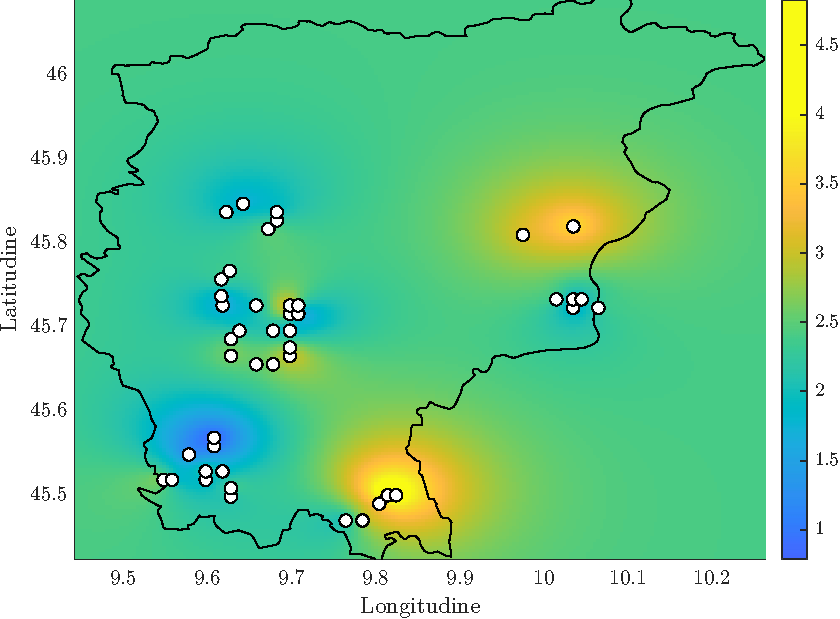
\includegraphics[width=\textwidth]{../Tesi/Immagini/2. Nuovo modello/Mappa potenziale, rho = 0}
			\end{figure}
		\end{column}
		\begin{column}[t]{0.5\linewidth}
			\centering
			$\rho = 0.5\cdot 10^{-2}$
			\begin{figure}
				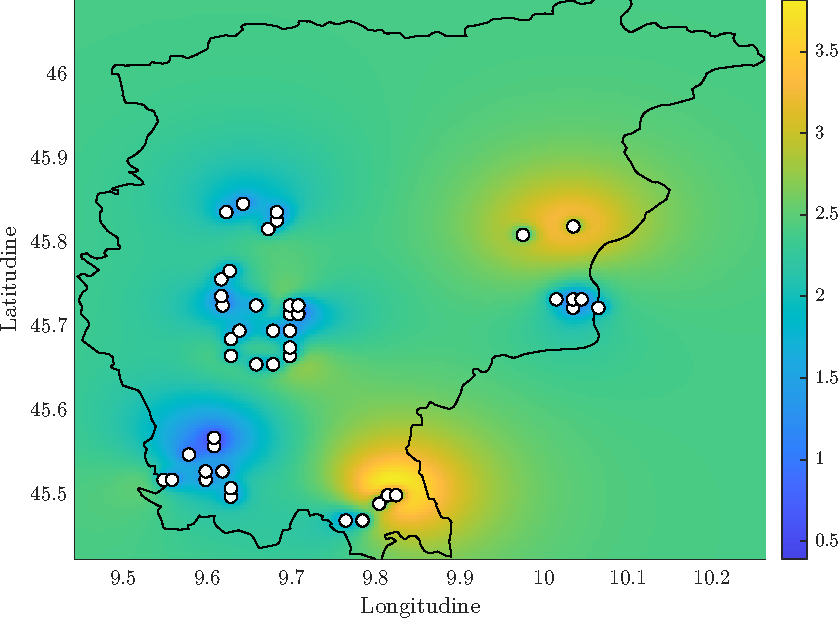
\includegraphics[width=\textwidth]{../Tesi/Immagini/2. Nuovo modello/Mappa potenziale, rho = 0.005}
			\end{figure}
		\end{column}
	\end{columns}

\end{frame}

\begin{frame}
	
	\begin{columns}[T]
		\begin{column}[t]{0.5\linewidth}
			\centering
			$\rho = 10^{-2}$
			\begin{figure}
				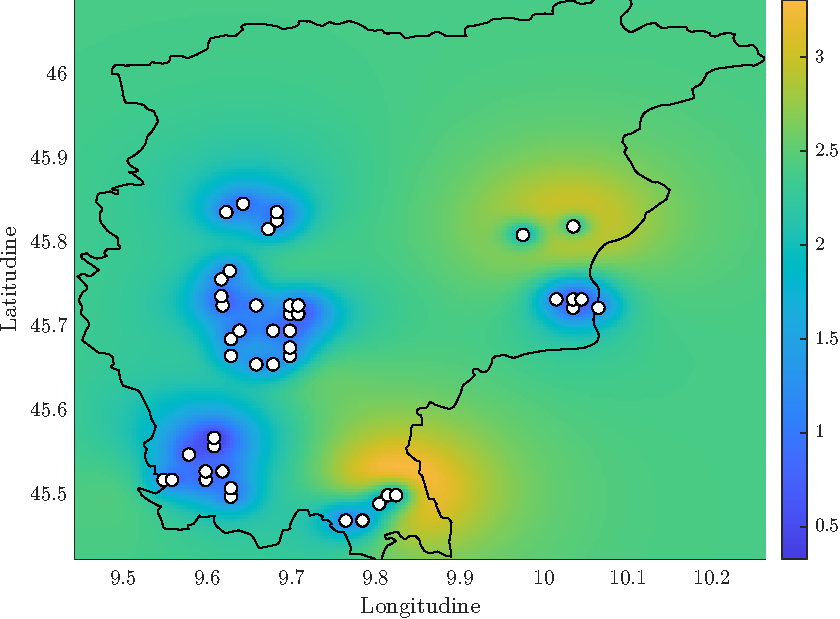
\includegraphics[width=\textwidth]{../Tesi/Immagini/2. Nuovo modello/Mappa potenziale, rho = 0.01}
			\end{figure}
		\end{column}
		\begin{column}[t]{0.5\linewidth}
			\centering
			$\rho = 1.5\cdot 10^{-2}$
			\begin{figure}
				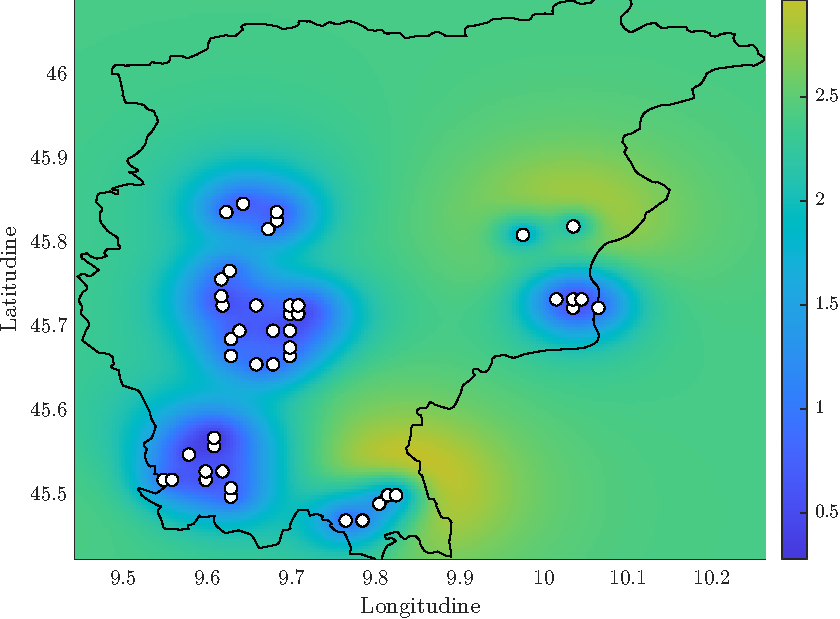
\includegraphics[width=\textwidth]{../Tesi/Immagini/2. Nuovo modello/Mappa potenziale, rho = 0.015}
			\end{figure}
		\end{column}
	\end{columns}
	
\end{frame}
	\section[Stima EM del modello fp-HDGM]{Stima EM del modello fp-HDGM}

\begin{frame}
	\frametitle{Obiettivo della stima EM}
	\justifying
	
	Sia:
	\begin{equation*}
		\boldsymbol{\theta} = \left(\boldsymbol{c}_\epsilon^\top, \boldsymbol{c}_\beta^\top, \mathbf{g}^\top, \mathbf{v}^\top, \boldsymbol{\lambda}^\top, \textcolor{red}{\rho}\right)^\top
	\end{equation*}
	il vettore dei parametri. 
	\newline \par L'obiettivo dell'\textbf{algoritmo Expectation-Maximization (EM)} è determinare, mediante un processo iterativo, la stima a massima verosimiglianza $\boldsymbol{\theta}_{MLE}$ \textbf{in presenza di dati mancanti}, in questo caso la componente latente $\mathbf{z}(\mathbf{s}, t)$.
\end{frame}

\begin{frame}
	\frametitle{I passi dell'algoritmo}
	\justifying
	
	Ogni iterazione dell'algoritmo EM consiste in due passi:
	\begin{itemize}
		\justifying
		\item \textbf{passo E}: a partire dalla stima corrente dei parametri $\boldsymbol{\theta}_n$ e dai dati disponibili $\mathbf{y}$, quelli mancanti vengono prima stimati e poi impiegati per determinare il \textit{valore atteso condizionato} $Q(\boldsymbol{\theta},\boldsymbol{\theta}_n)$, una semplificazione della stima corrente della funzione di verosimiglianza $L(\boldsymbol{\theta}|\boldsymbol{\theta}_n)$, ovvero $l(\boldsymbol{\theta}|\boldsymbol{\theta}_n)$;
		\item \textbf{passo M}: $Q(\boldsymbol{\theta},\boldsymbol{\theta}_n)$ viene ottimizzata per determinare $\boldsymbol{\theta}_{n+1}$, assumendo che i dati mancanti siano noti. Le stime di questi, ottenute precedentemente nel passo E, sono utilizzate al posto dei dati mancanti effettivi.
	\end{itemize}
\end{frame}

\begin{frame}
	\frametitle{La funzione di verosimiglianza}
	
	\begin{equation*}
		\begin{split}
			-2\ln L(\boldsymbol{\theta}; Y, Z, X) & =  T\ln|\Sigma_\epsilon\left(\textcolor{black}{\mathbf{c}_\epsilon}\right)| \\
			& + \textcolor{red}{\sum_{t=1}^{T} \left(H^{-1}(\rho)\cdot\mathbf{y}_t - \boldsymbol{\mu}_t(\mathbf{c}_\beta)\right)^\top\Sigma_\epsilon^{-1}\left(H^{-1}(\rho)\cdot\mathbf{y}_t - \boldsymbol{\mu}_t(\mathbf{c}_\beta)\right)} \\
			& + \ln|\Sigma_0| \\
			& + (\mathbf{z}_0 - \boldsymbol{\mu}_0)^\top\Sigma_0^{-1}(\mathbf{z}_0 - \boldsymbol{\mu}_0) \\
			& + T\ln |\Sigma_\eta(\textcolor{black}{\mathbf{v},\boldsymbol{\lambda}})| \\
			& + \sum_{t=1}^{T}\left(\mathbf{z_t}-\tilde{G}(\textcolor{black}{\mathbf{g}})\cdot\mathbf{z}_{t-1}\right)^\top\Sigma_\eta^{-1}(\textcolor{black}{\mathbf{v},\boldsymbol{\lambda}})\left(\mathbf{z_t}-\tilde{G}(\textcolor{black}{\mathbf{g}})\cdot\mathbf{z}_{t-1}\right)
		\end{split}
		\label{eq_fin_verosimiglianza}
	\end{equation*}
	
\end{frame}
	\section{Caso di studio}
\begin{frame}
	\frametitle{Descrizione del Dataset}
	\centering
	
	\begin{itemize}
		\justifying
		\item \textbf{Variabile dipendente}: l'oggetto del caso di studio consiste nel numero di ritiri orari di biciclette presso le stazioni della rete di bike sharing;
		\item \textbf{Variabili meteorologiche}: Covariate spazio-invarianti come temperatura percepita, piovosità, visibilità orizzontale, velocità del vento e copertura nuvolosa;
		\item \textbf{Variabili spaziali}: Covariate tempo-invarianti quali la distanza dalla stazione ferroviaria più vicina e la densità demografica nella zona circostante.
		\item \textbf{Variabili dummy}: Eventi come il lockdown COVID-19, il ritorno alla vita quotidiana post-lockdown, i weekend e le festività federali sono modellati come variabili categoriche binarie.
	\end{itemize}	
\end{frame}

\begin{frame}
	\centering
	\begin{columns}[T]
		\begin{column}[t]{0.5\linewidth}
			\centering
			\begin{figure}
				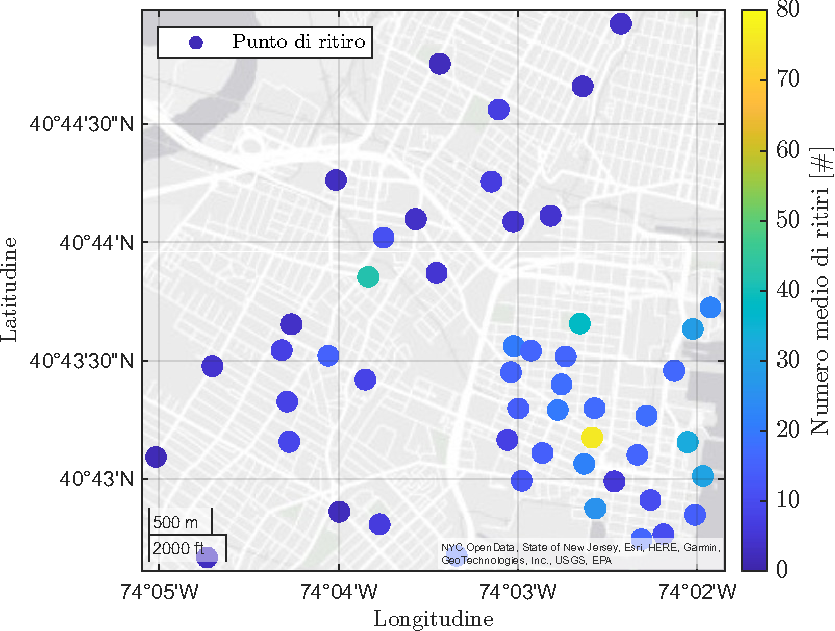
\includegraphics[width=\textwidth]{../Tesi/Immagini/4. Caso di studio/Mappe/Mappa ritiri, inverno}
			\end{figure}
		\end{column}
		\begin{column}[t]{0.5\linewidth}
			\centering
			\begin{figure}
				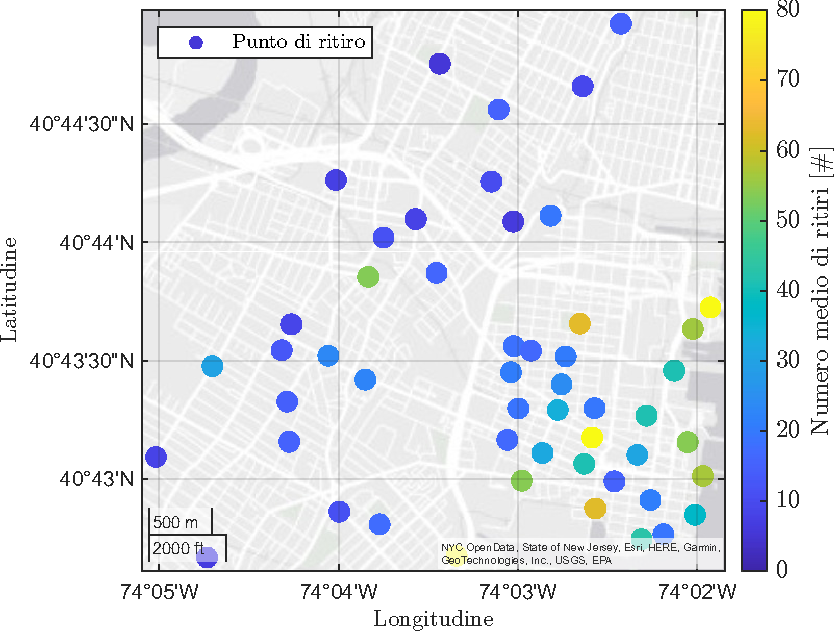
\includegraphics[width=\textwidth]{../Tesi/Immagini/4. Caso di studio/Mappe/Mappa ritiri, estate}
			\end{figure}
		\end{column}
	\end{columns}
	\textit{Distribuzione spaziale del numero medio di ritiri giornaliero presso le 51
	stazioni, in inverno (sinistra) e in estate (destra)}.
\end{frame}
\begin{frame}
	\centering
	\begin{columns}[T]
		\begin{column}[t]{0.5\linewidth}
			\centering
			\begin{figure}
				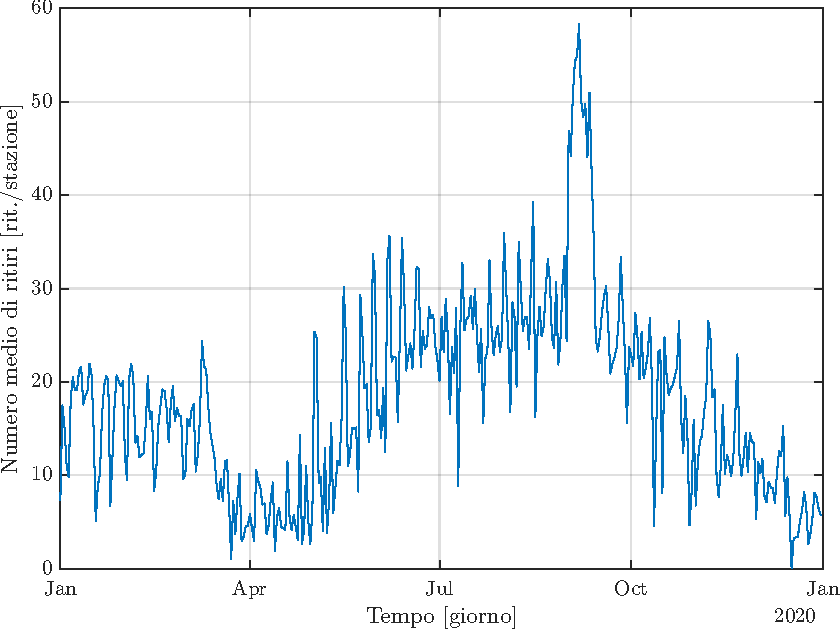
\includegraphics[width=\textwidth]{../Tesi/Immagini/4. Caso di studio/Serie storiche/Ritiri giornalieri}
			\end{figure}
		\end{column}
		\begin{column}[t]{0.5\linewidth}
			\centering
			\begin{figure}
				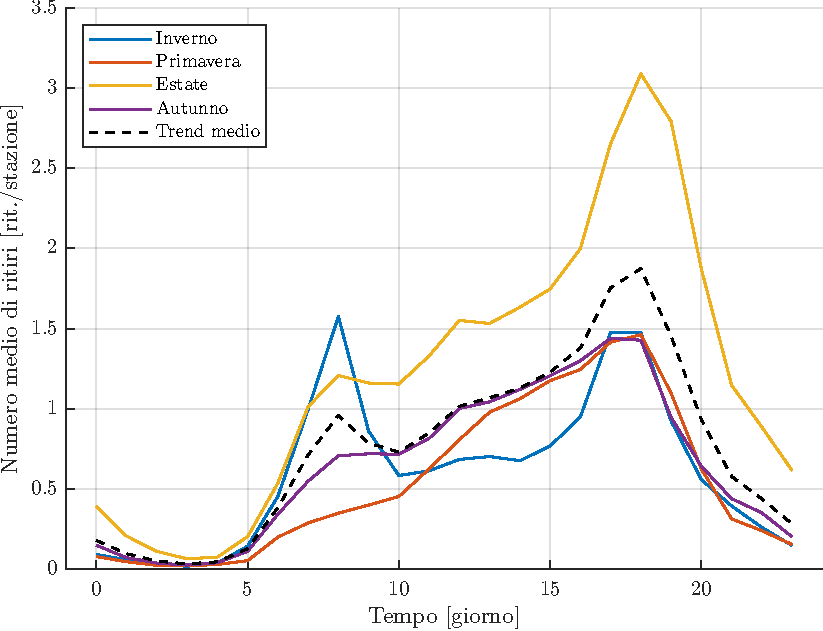
\includegraphics[width=\textwidth]{../Tesi/Immagini/4. Caso di studio/Serie storiche/Ritiri orari}
			\end{figure}
		\end{column}
	\end{columns}
	\textit{Andamento giornaliero (sinistra) e orario (destra) del numero medio di noleggi al variare
	della stagione.}
\end{frame}

\begin{frame}
	\centering
			\begin{figure}
				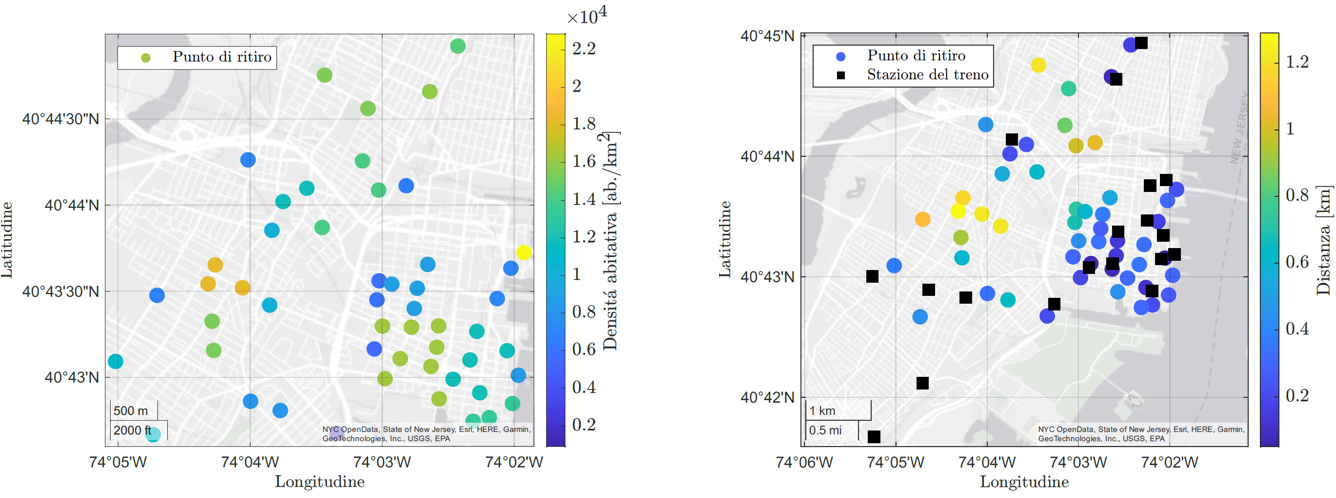
\includegraphics[width=\textwidth]{../Tesi/Immagini/4. Caso di studio/Mappe/Mappa punti ritiro e stazioni treno e densita ab AGGREGATA}
			\end{figure}
	\textit{Mappe della densità abitativa nei pressi dei punti di ritiro (sinistra) e delle distanze dei punti di interscambio dalla stazione ferroviaria più vicina (destra).}
\end{frame}

\begin{frame}
	\frametitle{Metodologia}
	\centering
	\begin{enumerate}
		\justifying
		\item \textbf{cross-validazione con $k=5$ per determinare il valore del parametro $\rho$}: Al fine di determinare il $\rho$ ottimale, come metrica è stato impiegato il MSE:
			\begin{equation*}
			\begin{aligned}
				MSE &= \frac{1}{P}\sum_{i=1}^{k=5}\frac{1}{\text{card}(\mathcal{S}_{val})_i}\sum_{\mathbf{s}\in\mathcal{S}_{val}}^{}\sum_{t=1}^{T}\sum_{l\in\mathcal{L}}^{} (y(\mathbf{s}, l, t) - \hat{y}(\mathbf{s}, l, t))^2; \\
				P &= k\cdot T\cdot q;
			\end{aligned}
		\end{equation*}
		\item \textbf{scelta delle covariate più significative (model selection)}: l'obiettivo è visualizzare le spline per i parametri $\beta$ e i relativi intervalli di confidenza al fine di escludere i regressori poco significativi;

	\end{enumerate}	
\end{frame}
\begin{frame}
	\centering
	
	\begin{enumerate}
		\setcounter{enumi}{2}
		\justifying
		\item \textbf{validazione del modello finale tramite LOOCV}: per valutare la bontà complessiva del modello definitivo, è stato utilizzato il RMSE:
		\begin{equation*}
			RMSE_\mathbf{s} = \sqrt{\frac{1}{T\cdot q}\sum_{t=1}^{T}\sum_{l\in\mathcal{L}}^{} (y(\mathbf{s}, l, t) - \hat{y}(\mathbf{s}, l, t))^2}.
		\end{equation*}
		\item \textbf{previsione spaziale utilizzando il kriging}: è stato computato il volume di noleggi orario così definito:
		\begin{equation*}
			v(\mathbf{s}, l|\mathcal{T}) = \sum_{t}^{\mathcal{T}} \hat{y}(\mathbf{s}, l, t), \ \forall \mathbf{s}\in\mathcal{D}, \ \forall l\in\mathcal{H}, \mathcal{T} = [152, 213]\subset [1, 366].
		\end{equation*}
			Dopodiché, i \num{24} valori di $v(\mathbf{s}, l|\mathcal{T})$ sono stati così raggruppati:
		\begin{equation*}
			\bar{v}(\mathbf{s}, l|\mathcal{T})_i = \frac{1}{\text{card}(\mathcal{R}_i)}\sum_{j\in\mathcal{R}_i}^{}v(\mathbf{s}, j|\mathcal{T}), \ i=1\dots 6;
		\end{equation*}
	\end{enumerate}	
\end{frame}

\begin{frame}
	\frametitle{Analisi dei risultati}
	\centering
	\begin{figure}
		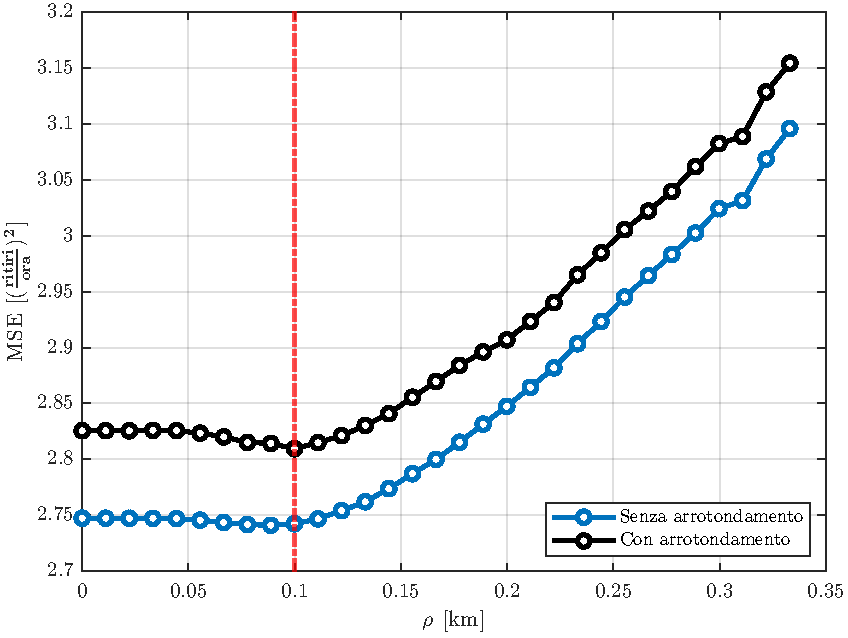
\includegraphics[height=130px]{../Tesi/Immagini/4. Caso di studio/Cross_validazione/MSE_rho_full_focus}
	\end{figure}
	\textit{Andamento del $MSE$ in cross-validazione con e senza arrotondamento al variare del parametro $\rho$.}
\end{frame}

\begin{frame}
	\centering
	\begin{figure}
		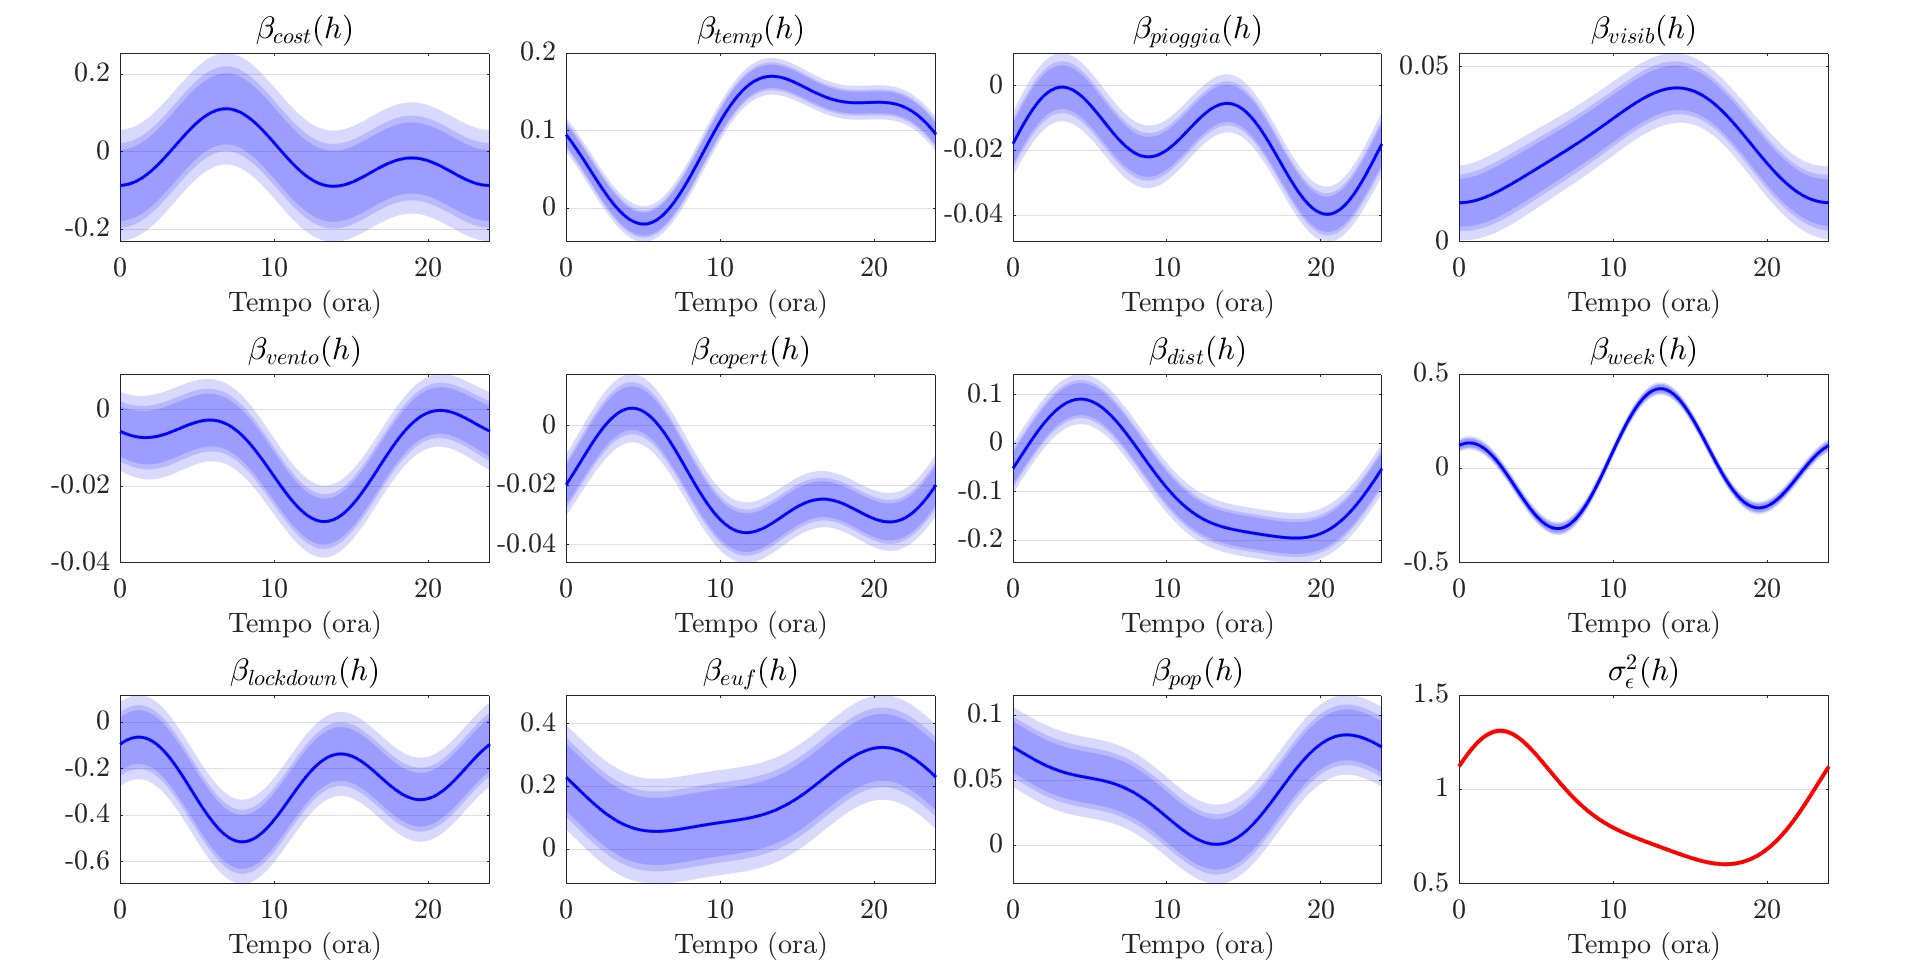
\includegraphics[height=170px]{../Tesi/Immagini/4. Caso di studio/Model selection/Trend spline, rho=100m}
	\end{figure}
	\textit{Spline di Fourier per i coefficienti $\boldsymbol{\beta}$ e rispettivi intervalli di confidenza}
\end{frame}

\begin{frame}
	\centering
	\begin{figure}
		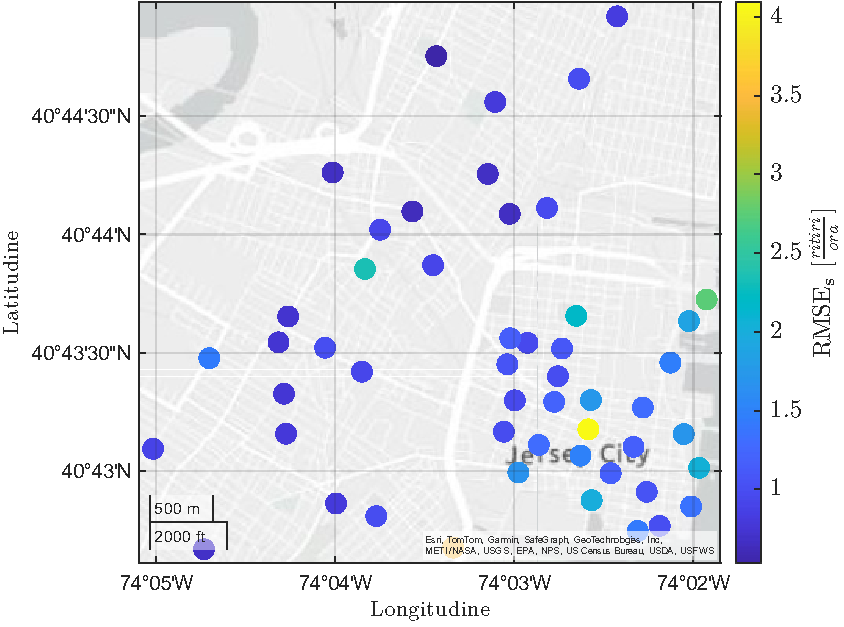
\includegraphics[height=170px]{../Tesi/Immagini/4. Caso di studio/LOOCV/RMSE_s}
	\end{figure}
	\textit{Mappa della distribuzione del $RMSE_\mathbf{s}$}
\end{frame}


\begin{frame}
	\centering
	\begin{columns}
		\begin{column}{0.33\linewidth}
			\centering
			\begin{figure}
				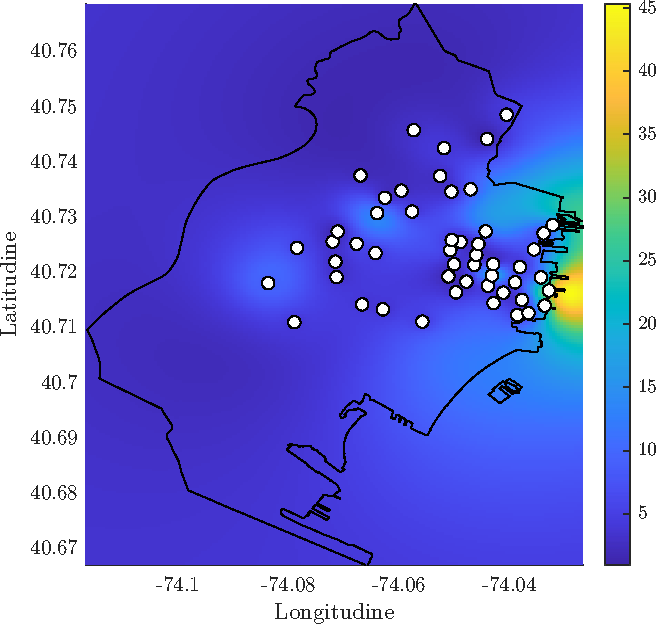
\includegraphics[width=\textwidth]{../Tesi/Immagini/4. Caso di studio/Kriging/Mappa volume, 1}
			\end{figure}
		\end{column}
		\begin{column}{0.33\linewidth}
			\centering
			\begin{figure}
				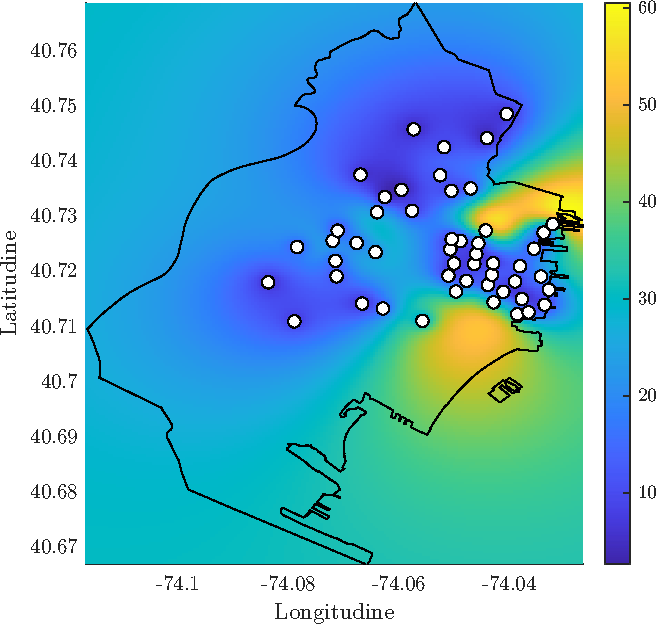
\includegraphics[width=\textwidth]{../Tesi/Immagini/4. Caso di studio/Kriging/Mappa volume, 2}
			\end{figure}
		\end{column}
		\begin{column}{0.33\linewidth}
			\centering
			\begin{figure}
				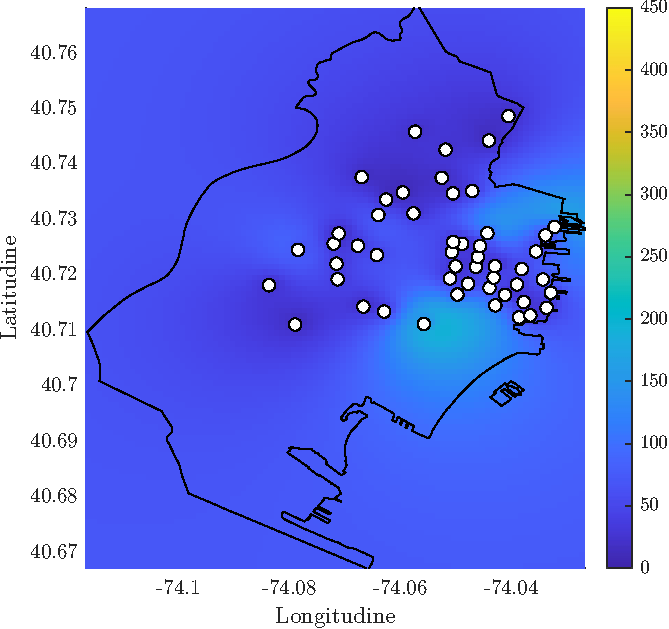
\includegraphics[width=\textwidth]{../Tesi/Immagini/4. Caso di studio/Kriging/Mappa volume, 3}
			\end{figure}
		\end{column}
	\end{columns}
	\textit{Volume del numero di ritiri previsti, raggruppati per fasce orarie: da 00:01 a 04:00 (sinistra), da 04:01 a 08:00 (centro), da 08:01 a 12:00 (destra).}
\end{frame}

\begin{frame}
	\centering
	\begin{columns}
		\begin{column}{0.33\linewidth}
			\centering
			\begin{figure}
				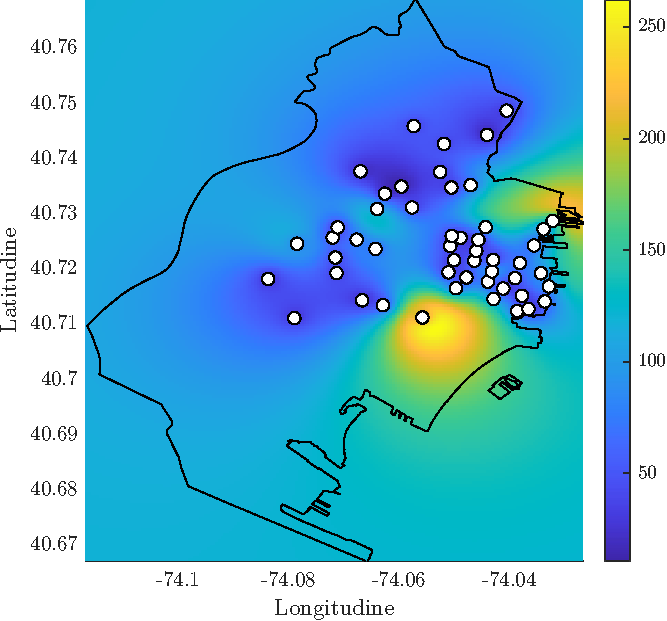
\includegraphics[width=\textwidth]{../Tesi/Immagini/4. Caso di studio/Kriging/Mappa volume, 4}
			\end{figure}
		\end{column}
		\begin{column}{0.33\linewidth}
			\centering
			\begin{figure}
				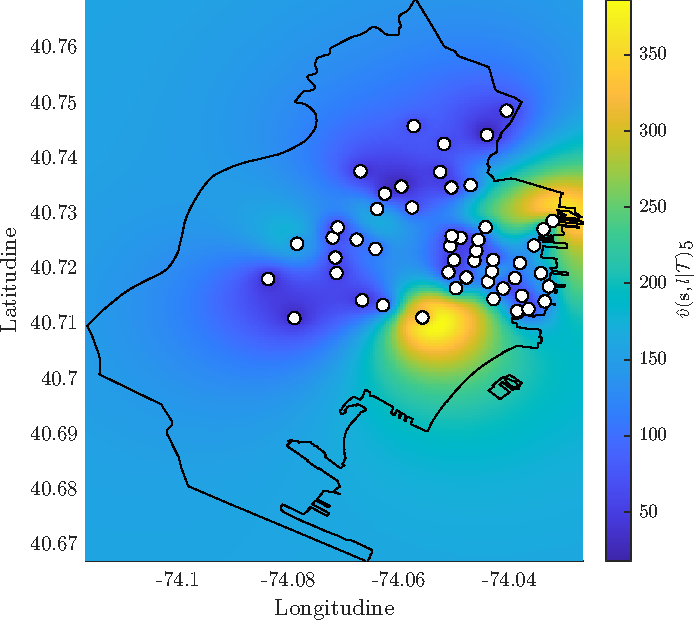
\includegraphics[width=\textwidth]{../Tesi/Immagini/4. Caso di studio/Kriging/Mappa volume, 5}
			\end{figure}
		\end{column}
		\begin{column}{0.33\linewidth}
			\centering
			\begin{figure}
				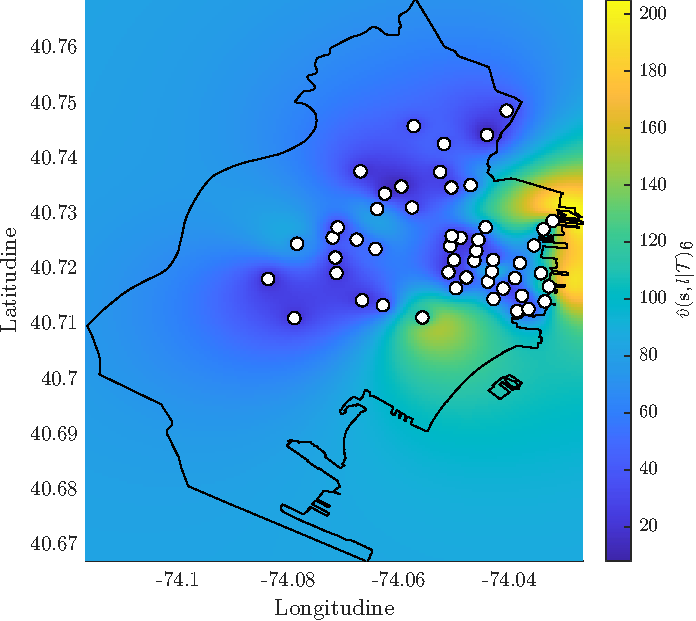
\includegraphics[width=\textwidth]{../Tesi/Immagini/4. Caso di studio/Kriging/Mappa volume, 6}
			\end{figure}
		\end{column}
	\end{columns}
	\textit{Volume del numero di ritiri previsti, raggruppati per fasce orarie: da 12:01 a 16:00 (sinistra), da 16:01 a 20:00 (centro), da 20:01 a 24:00 (destra).}
\end{frame}
	\section{Conclusioni}
\begin{frame}
	\frametitle{Conclusioni}
	\centering
	
	\begin{itemize}
		\justifying
		\item Il presente studio evidenzia il valore aggiunto del nuovo modello proposto nel campo della modellazione funzionale spazio-temporale, distinguendosi dal modello f-HDGM grazie all'introduzione del parametro di interazione spaziale $\rho$;
		\item una delle limitazioni riguarda il processo di stima del nuovo parametro, poiché la cross validazione richiede risorse computazionali significative;
	\end{itemize}	
\end{frame}

\begin{frame}
	\centering
	\begin{itemize}
		\justifying
		\item é necessaria la modifica dell'algoritmo EM affinché sia in grado di minimizzare anche la funzione $m(\rho)$, ma ciò richiede ulteriori sessioni di ricerca e sviluppo per affrontare questioni ancora aperte, come la verifica dell'identificabilità e l'inizializzazione corretta di $\rho$.		
		\item per migliorare l'analisi sul bike sharing, si potrebbe considerare l'utilizzo di un dataset pluriennale per catturare la componente stagionale del fenomeno e l'adozione di variazioni metodologiche come il clustering dei punti di ritiro per permettere la stima di modelli spazio-temporali locali, riducendo l'assunzione che il parametro $\rho$ sia spazio-invariante.
	\end{itemize}	
\end{frame}
	
\end{document}